\section{Searching}

When we search for data, we want to find the data as quickly as possible.

Searching through unorganized data must be $O(n)$, as we have to look at every element to find the data. This is called \textbf{linear / sequential search}.

This could be \textbf{not true for organized data}, where we can \textbf{gain information} about the data \textbf{without} looking at every element, such as with a sorted list.

We will focus on searching algorithms on a \textbf{sorted list} in this section.

\begin{definition}
    {Jump search}
    Works by:
    \begin{itemize}
        \item Access linearly every floor($\sqrt{n}$) elements
        \item If the element is greater than the target, go back to the previous jump
        \item Linearly search the elements in the jump
    \end{itemize}
    \textbf{Amount of comparisons} $=\frac{n}{\sqrt{n}} + \sqrt{n} - 1$

    \textbf{Time complexity:} $\Theta(\sqrt{n}) O(\sqrt{n})$
\end{definition}

\begin{definition}
    {Binary search}
    Works by:
    \begin{itemize}
        \item Start at the middle of the list
        \item If the element is greater than the target, search the left half
        \item If the element is less than the target, search the right half
    \end{itemize}

    \textbf{Time complexity:}  $\Theta(\log n) O(\log n)$

    Remember that the middle must be recalculated each time.
\end{definition}

\begin{theorem}
    {Interpolation search}
    An improved version of binary search. Instead of searching the middle, we search the \textbf{interpolated position} (probe) based on the target.

    \[ \text{probe} = \text{low} + \frac{(\text{high} - \text{low})}{(\text{A[high]} - \text{A[low]})} \times (\text{target} - \text{A[low]}) \]

    \textbf{Time complexity:} $\Theta(\log \log n) O(n)$

    \textbf{Note:} This is only effective when the data is \textbf{evenly distributed} (linear). Otherwise, it is not effective, such as when the data is exponential, resulting in $O(n)$ time complexity.
\end{theorem}

\section{Tree searching}

We can use a tree to search for data. BST and AVL trees guarentee $\Theta(\log n)$ time complexity, as we don't have to access every element to gain information about them.

This is built upon the idea of binary search.

\subsection{Binary search tree}

\begin{definition}
    {Binary search tree (BST)}
    A binary tree (two child nodes per node) that satisfies the following properties:
    \begin{itemize}
        \item Left node: key $\leq$ root.key
        \item Right node: key $>$ root.key
    \end{itemize}
    The height of a BST is $\log n$.
\end{definition}

\begin{theorem}
    {Time complexities}
    Consider the height of a BST:
    \begin{itemize}
        \item Min height: $\log_2 n + 1$
        \item Max height: $n$ (All nodes are in a straight line)
    \end{itemize}
    We can then conclude the time complexities for insert, search and delete is: $\Theta(\log n) O(n)$
\end{theorem}

\begin{theorem}
    {Traversal methods}
    The following are three recursive methods to traverse a tree:
    \begin{itemize}
        \item Pre-order: root$\to$left$\to$right
        \item In-order: left$\to$root$\to$right
        \item Post-order: left$\to$right$\to$root
    \end{itemize}
    Where you access the root and \textbf{recursively} trasverse the left and right subtrees. When we consider trees, we always think recursively.
\end{theorem}

To search for a node in a BST, we can simply captialized on the properties of the tree:
\begin{enumerate}
    \item Start at the root
    \item If the key is less than the root, go left
    \item If the key is greater than the root, go right
    \item Return if equal
\end{enumerate}
Remember, we always consider trees recursively.

\subsection{Balancing trees}

\begin{knBox}
    {The balance factor}
    \[B(n)=\text{left.height} - \text{right.height}\]

    A perfectly balanced tree has $B(n)=0$.
\end{knBox}

\begin{definition}
    {AVL tree}
    A self-balancing binary search tree where $|{B(n)}|\leq 1$.

    \textbf{Self-balancing} means that when modifying the tree, it will \textbf{rotate} the tree to \textit{fix imbalance}.
\end{definition}

\begin{theorem}
    {Time complexities}
    The time complexities for insert, search and delete in an AVL tree is $\Theta(\log n) O(\log n)$.
\end{theorem}

\begin{theorem}
    {Rotations}
    We rotate the tree to fix imbalance during insertions and deletions.

    A rotation is done by \textbf{shifting the root} of a subtree to the left or right.

    \begin{center}
        \begin{tabular}{|c|c|}
            \textbf{\underline{L}eft Rotation} & \textbf{\underline{R}ight Rotation} \\
            When: Right-heavy                  & When: Left-heavy                    \\
            \hline
            $B$: 2 -ve nodes from root         & $B$: 2 +ve nodes root               \\
            shift root to \underline{R}        & shift root to \underline{L}         \\
            \hline
            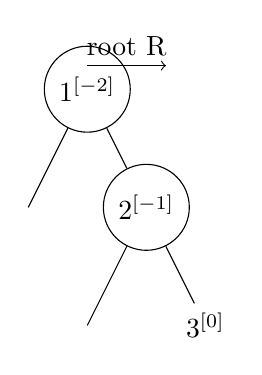
\begin{tikzpicture}[baseline=(current bounding box.center)]
                \node[circle, draw, minimum size=1cm]  {$1^{[-2]}$}
                child {}
                child {node[circle, draw, minimum size=1cm]  {$2^{[-1]}$}
                        child {}
                        child {node {$3^{[0]}$}}
                    };
                \draw[->] (0,0.3) -- (1,0.3) node[midway, above] {root R};
            \end{tikzpicture}
            $\implies$
            \begin{tikzpicture}[baseline=(current bounding box.center)]
                \node {2}
                child {node {1}
                    }
                child {node {3}
                    };
            \end{tikzpicture}
                                               &

            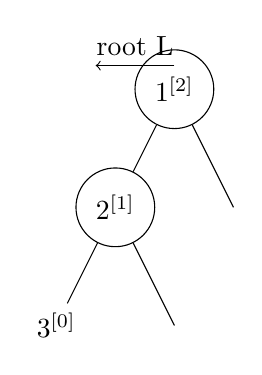
\begin{tikzpicture}[baseline=(current bounding box.center)]
                \node[circle, draw, minimum size=1cm]  {$1^{[2]}$}
                child {node[circle, draw, minimum size=1cm]  {$2^{[1]}$}
                        child {node {$3^{[0]}$}}
                        child {}
                    }
                child {};
                \draw[->] (0,0.3) -- (-1,0.3) node[midway, above] {root L};
            \end{tikzpicture}
            $\implies$
            \begin{tikzpicture}[baseline=(current bounding box.center)]
                \node {2}
                child {node {3}
                    }
                child {node {1}
                    };
            \end{tikzpicture}
        \end{tabular}
    \end{center}

    For cases where $B$ is not 2 nodes of the same sign from root, we need to \textbf{consider the subtree} and perform a rotation on it, then rotate the root. This is a \textbf{double rotation}.

    \begin{center}
        \begin{tabular}{|c|c|}
            \textbf{R-L Rotation}                                      & \textbf{L-R Rotation}                                      \\
            When: Right-left heavy                                     & When: Left-right heavy                                     \\
            \hline
            $B$: +ve node, -ve node                                    & $B$: -ve node, +ve node                                    \\
            shift subtree root to \underline{L}, root to \underline{R} & shift subtree root to \underline{R}, root to \underline{L} \\
            \hline
            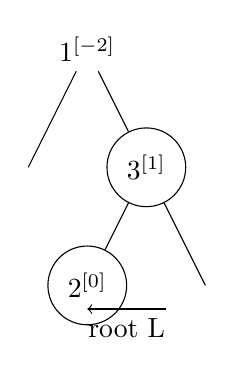
\begin{tikzpicture}[baseline=(current bounding box.center)]
                \node {$1^{[-2]}$}
                child {}
                child {node[circle, draw, minimum size=1cm]  {$3^{[1]}$}
                        child {node[circle, draw, minimum size=1cm]  {$2^{[0]}$}}
                        child {}
                    };
                \draw[->] (1,-3.3) -- (0,-3.3) node[midway, below] {root L};
            \end{tikzpicture}
            $\implies$
            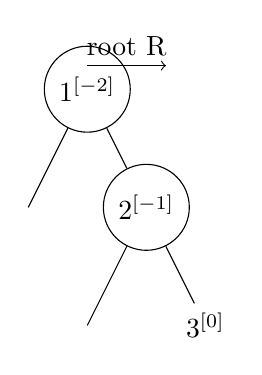
\begin{tikzpicture}[baseline=(current bounding box.center)]
                \node[circle, draw, minimum size=1cm]  {$1^{[-2]}$}
                child {}
                child {node[circle, draw, minimum size=1cm]  {$2^{[-1]}$}
                        child {}
                        child {node {$3^{[0]}$}}
                    };
                \draw[->] (0,0.3) -- (1,0.3) node[midway, above] {root R};
            \end{tikzpicture}
                                                                       &
            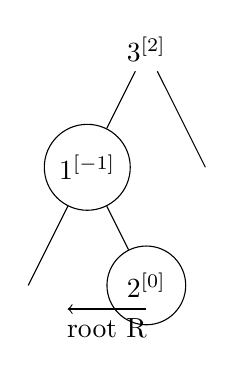
\begin{tikzpicture}[baseline=(current bounding box.center)]
                \node {$3^{[2]}$}
                child {node[circle, draw, minimum size=1cm]  {$1^{[-1]}$}
                        child {}
                        child {node[circle, draw, minimum size=1cm]  {$2^{[0]}$}}
                    }
                child {};
                \draw[->] (0,-3.3) -- (-1,-3.3) node[midway, below] {root R};
            \end{tikzpicture}
            $\implies$
            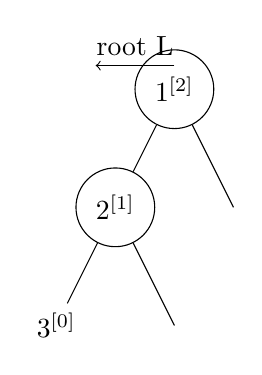
\begin{tikzpicture}[baseline=(current bounding box.center)]
                \node[circle, draw, minimum size=1cm]  {$1^{[2]}$}
                child {node[circle, draw, minimum size=1cm]  {$2^{[1]}$}
                        child {node {$3^{[0]}$}}
                        child {}
                    }
                child {};
                \draw[->] (0,0.3) -- (-1,0.3) node[midway, above] {root L};
            \end{tikzpicture}
        \end{tabular}
    \end{center}
\end{theorem}